\chapter{Implementation}\label{chapter:implementation}
% This chapter describes the implementation of component X. Three systems were chosen
% as reference implementations: a desktop version for Windows and Linux PCs, a Windows
% Mobile version for Pocket PCs and a mobile version based on Android.
This chapter describes the implementation of the motey engine as well as the deployment and capability logic.
Used technologies, libraries and tools, as well as custom components would be presented and the functionality will be demonstrated.
Thereby challenges and problems during the development of the plugins will be shown and the solutions will be discussed.

\section{Environment}
To motey engine is designed to be exectued on low-power devices like a Raspberry Pi.
The following software is required to execute the whole software stack.
\begin{itemize}
  \item Ubuntu version 14.10 or higher
  \item Python 3.5 or newer
  \item Docker 17.3 or higher
\end{itemize}
On hardware side motey will be tested on Raspberry Pis type 2 B or newer.
Depending on the amount and type of the executed Docker images, the hardware specifications may can vary.
% TODO: installation instructions?

\section{Project structure}

% The implementation is seperated into 2 distinguished eclipse projects as depicted in
% figure 5.1.
% The following listing briefly describes the single packages of both projects in alphabetical
% order to give an overview of the implementation:
Beside the main folder with the motey engine, the project contains several directories with helpfull scripts and tools.
A brief overview about the project structure will givin in this section.
A detailed explanation of all files will be omitted, as this would exceed the scope of the thesis.

\begin{itemize}
  \item{\textbf{Directory: ./}} has all the necessary configuration files for the different services.
  \begin{itemize}
    \item{\textbf{File: .dockerignore}} is used during the build process of a Docker image. Excludes several folders during the build phase.
    \item{\textbf{File: .editorconfig}} contains informations for \acp{IDE} and editors to guarantee a consistent coding style.
    \item{\textbf{File: .gitignore}} excludes file to be tracked by the version control system git.
    \item{\textbf{File: .travis.yml}} is used by the continuous integration tool Travis CI.
    \item{\textbf{File: AUTHORS.rst}} a list of all contributors.
    \item{\textbf{File: CHANGELOG.rst}} this document records all notable changes to the motey engine.
    \item{\textbf{File: LICENSE}} the License of the project (Apache License Version 2.0).
    \item{\textbf{File: main.py}} can be used to start motey in debug mode.
    \item{\textbf{File: MANIFEST.in}} contains meta information for the Python setup procedure.
    \item{\textbf{File: README.rst}} file to show up a short documentation on github and will act as the starting point of the project.
    \item{\textbf{File: setup.py}} will be used to install motey on a local machine.
  \end{itemize}
  \item{\textbf{docs:}} contains the files to create and display the documentation resources.
  \begin{itemize}
    \item{\textbf{Directory: source}} has all the files to autogenerate the documentation files from the source code.
    \item{\textbf{File: Makefile}} this file was created by the Sphinx documentation tool. By executing the \textit{Makefile} the related documentation files will be created.
  \end{itemize}
  \item{\textbf{motey:}} this folder contains the motey main engine. It is the main Python project. The whole structure will be explained on the next pages in detail.
  \item{\textbf{motey-docker-image:}} has all the necessary files to create a Docker image.
  \begin{itemize}
    \item{\textbf{File: Dockerfile}} to build the Docker image. Is analogous to a Makefile but can only be used by the Docker engine.
    \item{\textbf{File: setup.sh}} will be executed during the build phase and will install necessary tools and can executed command line instructions.
    \item{\textbf{File: requirements.txt}} a list with the Python requirements which are necessary to run the motey engine and which should be installed during the build phase via pip.
  \end{itemize}
  \item{\textbf{resources:}} is a resource folder for the github documentation. Will only be used by the \textit{README.rst} file in the root folder and the \textit{index.rst} file in the docs\/source folder.
  \item{\textbf{samples:}} contains some samples to test the functionality of the motey engine. Is primarily a playground to test new functions.
  \item{\textbf{scripts:}} some scripts which will be executed frequently during the development phase.
  \begin{itemize}
    \item{\textbf{Folder: config}} configuration files which could be used for the mosquitto \ac{MQTT} broker Docker image.
    \item{\textbf{File: addcapability.py}} can be used to add new capability entries to a running motey instance.
    \item{\textbf{File: start\_test\_setup.sh}} can be used to start a new local Docker test cluster.
  \end{itemize}
  \item{\textbf{tests:}} contains all the unit test which are executed by the continuous integration script and the Python setup procedure.
  \item{\textbf{webclient:}} this folder contains the \ac{GUI} for the motey engine. Will also be described on the next pages in detail.
\end{itemize}

\section{Used external libraries}
This section will show up some of the most important libraries used in the motey engine.
Each library will be introduced briefly and the reason for using it in the project will be shown.

\paragraph{daemonize} allows to run a services as a daemon process.
It is made exclusively for Unix-like systems.
The library will create a pid file after starting the service.
In the motey engine, the file path can be configured via a configuration file.
The daemon process can be controlled via a command line interface.
\begin{listing}[H]
  \begin{minted}{shell}
  Motey command line tool.

  Usage:
    motey start
    motey stop
    motey restart
    motey -h | --help
    motey --version

   Options:
     -h, --help       Show this message.
     --version        Print the version.
  \end{minted}
  \caption{Command line interface documentation for the daemon process}
  \label{code:cli-tool}
\end{listing}
After the motey engine is installed via the setup script, this command line tool will be available in the terminal.

\paragraph{dependency-injector} is a microframework for \acf{DI} in Python.
The \ac{DI} pattern allows to move the responsibility for creating a dependency from the concrete objects to a factory or a framework which creates the dependency graph.
This grants the single responsibility concept for classes and makes the whole code base much easier to unit test, because a dummy object can be passed to the constructor of the class.
It is also possible to mocked the object with the help of a mocking library.
To realize \ac{DI} in the Motey a so called \textit{app\_module.py} was created which uses the \textit{dependency-injector} framework to create the dependency graph.
Several \ac{IoC} containers are created in that file and will be used by the framework to generate the glue code.
Most of the injected components are instanciated as singleton objects to guarantee that there is only one active instance of that component at a time.
The implementation of the singleton design pattern is also provided by the framework.
Listing \ref{code:app-module} demonstrates the implementation of such an \ac{IoC} container.
\begin{listing}[H]
  \begin{minted}{python}
  class DIRepositories(containers.DeclarativeContainer):
      capability_repository = providers.Singleton(CapabilityRepository)
      nodes_repository = providers.Singleton(NodesRepository)
      service_repository = providers.Singleton(ServiceRepository)
  \end{minted}
  \caption{Extract of a sample \ac{IoC} container from the app\_module.py}
  \label{code:app-module}
\end{listing}

\paragraph{Docker \ac{SDK}}
The Docker Python library is a wrapper around the Docker command line tool.
Every command that can be executed with this tool can also be executed from any python code.
In the initializing phase the library will connect to the Docker Engine \ac{API} and will perform all the actions through them.
This can be realized via an \ac{URL} to the \ac{REST} \ac{API} or via an unix system socket connection.
In the motey engine the second method will be used, but can be replaced without any limitations.
The library is used as a \ac{VAL} plugin and will be automatically loaded at runtime via the VALManager and the Yapsy plugin system.

\paragraph{Flask} is a framework to create web applications.
Flask does not provide any templating or database engine, nor does it enforce a specific file structure.
Instead it will support extensions to add functionalities like that so that the developer can choose the tools of choice.\autocite[cf.]{Flask:Documentation:Foreword}
Nevertheless Flask is production ready and is used in several big projects like Pinterest\autocite{Quora:Pinterest:Flask} or Twilio\autocite{Twilio:Flask}.

Flask can use so called \textit{Blueprint} to configure new routes in the webserver.
A Blueprint is basically a Python class that can define methods like \textit{get} or \textit{post} to handle the specific \ac{HTTP} verbs.
This is useful to create valid \ac{HATEOAS} \ac{REST} \acp{API}.
Each Blueprint will be represented by an \ac{URL} endpoint.

Listing \ref{code:flask-blueprint} illustrates the implementation of all \ac{API} endpoints in motey.
\begin{listing}[H]
  \begin{minted}{python}
    def configure_url(self):
      self.webserver.add_url_rule('/v1/capabilities', view_func=Capabilities.as_view('capabilities'))
      self.webserver.add_url_rule('/v1/nodestatus', view_func=NodeStatus.as_view('nodestatus'))
      self.webserver.add_url_rule('/v1/service', view_func=Service.as_view('service'))
      self.webserver.add_url_rule('/v1/nodes', view_func=Nodes.as_view('nodes'))
  \end{minted}
  \caption{Implementation of all Flask \ac{API} endpoints in motey}
  \label{code:flask-blueprint}
\end{listing}

In line 2 a new endpoint will be add via the \textit{add\_url\_rule} to the Flask webserver.
The first parameter indicates the endpoint \ac{URL} and the second parameter \textit{view\_func} represents the Blueprint class, in this case \textit{Capabilities}.
To pass them over, the Blueprint has to be converted to a Flask view by using the \textit{as\_view} method.
The other endpoints are implemented equivalent.

\paragraph{Logbook} is a small loging library that helps to standardize the output of log messages.
It helps to address several output methods like the terminal, a file or even emails and linux desktop notifications.
The style of the resulting message can be easily configured and it can be integrated into several other libraries.
In addition to that, Logbook has a build-in support for messaging libraries like ZeroMQ, RabbitMQ or Redis.
This allows to distribute log messages on heavily distributed systems like a huge node cluster.
It was created by Armin Ronacher the crator of Flask and Georg Brandl the creator of Sphinx, both are tools that are used in motey.
Unfortunately there is no build-in support in Flask yet.
In the motey engine Logbook will be extended by a wrapper class to simplify the configuration of the tool.
The output folder for the log messages can be configured via the global config file and will be loaded in the constructor of the wrapper class.
If the folder path does not exist, it will be created.

\paragraph{paho-mqtt} is the python implementation of the Eclipse paho\footnote{\url{http://www.eclipse.org/paho}} project that is basically the implementation of the \ac{MQTT} messaging protocols, which was already described in section \ref{section:MQTT}.
The libarary allows to connect to a \ac{MQTT} broker like the Mosquitto broker.
It also comes with a variety of helper methods to eases the usage.
A wrapper class to centralize the usage of the library was created and the configuration as well as some smaller improvements was made in this wrapper class.
The whole configuration of the client can be configures via the global config file again.
Furthermore the routes are managed in the wrapper and a after connect handler was implemented.
It will be used to perform actions after a successfully created connection to the broker was made and all subscriptions to topics are done.
This helps to realize the node discovery mechanism described in section \ref{subsection:CommunicationLayer}.

\paragraph{pyzmq} is the third important communication library.
It is the official Python binding for ZeroMQ.
A detailed description of ZeroMQ can be found in section \ref{section:ZeroMQ} and in the great ZeroMQ guide at \url{http://zguide.zeromq.org/page:all}.
This library is also abstracted by wrapper class in motey.
This helps to configure the ZeroMQ server and register all necessary nodes.
A detailed explanition of the internals will be discussed in the following section \ref{subsection:implementation-communication-layer}.

\paragraph{Sphinx} is a tool to autogenerate a documentation out of the source code documentation.
It supports several output formats like \ac{HTML}, \LaTeX\ or ePub and is the defacto standard in Python.
The documentation hosting platform Read the Docs\footnote{\url{http://readthedocs.org}} completely supports Sphinx documentations.
As mentioned before the Makefile in the docs folder will be used to autogenerate the documentation files.
The scripts handles also the deployment of the documentation.
Therefore the files will be generated, the current branch will be switched to \textit{gh-pages}, which is be used to display the github page at \url{https://neoklosch.github.io/Motey/} and a new commit will be pushed with an autogenerated commit message.
Finally the branch will be switched back again.
Read the Docs has an active webhook that builds the builds the current documentation and display them at \url{http://motey.readthedocs.io}.
The documentation is also used as the official github page of the project at \url{https://neoklosch.github.io/Motey}.

\paragraph{TinyDB} is a wrapper to implement a lightweight document oriented database.
It stores the data into single \ac{JSON} files.
The location can be configured via the global config file.
TinyDB only supports very basic functionalities.
For example it does not support indexes or relationships and it is not optimised concerning performance.
But it is easy to use, has no execution overhead and it performs very well on smaller datasets.
The main purpose of the library is to be used for small apps where database server like MySQL\footnote{\url{https://www.mysql.com}} or MongoDB\footnote{\url{https://www.mongodb.com}} will be a huge overhead.
Furthermore TinyDB has several extension to add more functionalities like indexing or caching.
It also allows to easily extend the library with custom middlewares and extensions.
In the motey engine, TinyDB is used in every \textit{repository} to decorate the usage of the library.
Thereby the used library can easily replaced by a different one, without refactoring several class in the project.
A detailed discription of the implementation will be shown in \ref{subsection:impl-data-layer}.

\paragraph{Yapsy} is a plugin system that was designed to make an application easily extensible and should also be easy to use.
Several plugin systems are too complicated for a basic usage or have a huge dependency overhead.
Yapsy claims to be different, because it is written in pure Python and can be used with only a few lines of code.
In the motey engine all \ac{VAL} plugins will be loaded via Yapsy.
An extract of the VALManager with the method to register the plugins, is shown in listing \ref{code:yapsy-register-plugins}.
\begin{listing}[H]
  \begin{minted}{python}
  def register_plugins(self):
    self.plugin_manager.setPluginPlaces(
      directories_list=[absolute_file_path("motey/val/plugins")]
    )
    self.plugin_manager.collectPlugins()
    for plugin in self.plugin_manager.getAllPlugins():
        plugin.plugin_object.activate()
  \end{minted}
  \caption{Extract of the VALManager with the method to register plugins}
  \label{code:yapsy-register-plugins}
\end{listing}
In motey there is a specific folder where all images has to be located (line 2).
This could be extended in the future if necessary.
Afterwards all the valid plugins will be loaded and activated (line 3).
Finally for all activated plugins the \textit{activate} method will be executed, which is a custom implementation to call some functions after activating a plugin (line 4 and 5).
All plugins can be used via the \textit{self.plugin\_manager}.

\section{Important Implementation Aspects}
% Do not explain every class in detail. Give a short introduction about the modules or
% the eclipse projects. If you want to explain relevant code snippets use the ’lstlisting’ tag
% of LaTeX. Put only short snippets into your thesis. Long listing should be part of the
% annex.

% You can also compare different approaches. Example: Since the implementation based
% on X failed I choosed to implement the same aspect based on Y. The new approach
% resulted in a much faster ...

% Core samt daemon erklären
\doit

\subsection{motey engine}
% klassendiagramm
% einzelne Pakete erklären

\subsection{Data layer}
\label{subsection:impl-data-layer}
As mentioned before TinyDB is used as the database engine of choice.
To abstract TinyDB from the rest of the source code, the repository pattern will be used.
Each content type has its own database and also a related repository.
Every repository is inheriting from a \textit{base repository}.
This repository is used to implement some default methods and will also create the database path in the constructor if it is necessary.
The repositories are pretty similar implementation-wise.
They only differ in using different models and have some specific methods to be executed.
These models are used to represent the related \ac{JSON} objects.
Therefore each model have a static transform method to convert \ac{JSON} objects to the related model.
The models folder also contains a file called \textit{schemas.py}.
This file contains the validation schemas for the different \ac{YAML} and \ac{JSON} objects that could be received by the nodes.
A library called \textit{jsonschema} is used to validate the objects based on such a schema.
An example for a schema is shown in listing \ref{code:capability-schema}.
\begin{listing}[H]
  \begin{minted}{python}
  capability_json_schema = {
      "type": "array",
      "items": {
          "type": "object",
          "properties": {
              "capability": {
                  "type": "string"
              },
              "capability_type": {
                  "type": "string"
              }
          },
          "required": ["capability", "capability_type"]
      }
  }
  \end{minted}
  \caption{Capability JSON validation schema}
  \label{code:capability-schema}
\end{listing}
The jsonschema library allows to validate the type of an entry (line 2, 7 and 10) and also if the fields are required or optional (line 13).
This guarantees that only valid objects will be processed.

Another data layer component is the configuration reader.
This is implemented with the default Python \textit{configparser}.
The parsed configuration is only keept in memory.
The configuration file for the whole project is stored in the \textit{motey/configuration} folder and is called config.ini.
Listing \ref{code:config-ini} show the sample content of that file.
\begin{minted}{python}
[GENERAL]
app_name = Motey
pid = /var/run/motey.pid

[LOGGER]
name = Motey
log_path = /var/log/motey/
file_name = application.log

[WEBSERVER]
ip = 0.0.0.0
port = 5023

[MQTT]
ip = 172.18.0.3
port = 1883
keepalive = 60
username = neoklosch
password = neoklosch

[DATABASE]
path = /opt/Motey/motey/databases

[ZEROMQ]
capability_engine = 5090
capabilities_replier = 5091
deploy_image_replier = 5092
image_status_replier = 5093
image_terminate_replier = 5094
\end{minted}
\captionof{listing}{Example of the config.ini file\label{code:config-ini}}
\vspace{0.5cm}
Different sections can be seperated by squared brackets like \textit{[GENERAL]} like on line 1.
The entries are simple key-value pairs.
Line 3 for example set the path to the used pid file.
The usage of the configreader is shown in listing \ref{code:configreader-example}.

\begin{listing}[H]
  \begin{minted}{python}
  from motey.configuration.configreader import config

  daemon = Daemonize(
      app=config['GENERAL']['app_name'],
      pid=config['GENERAL']['pid'],
      action=run_main_component
  )
  \end{minted}
  \caption{Example of the usage of the configreader}
  \label{code:configreader-example}
\end{listing}
The configuration object must be imported from the configreader module (see line 1) and can be used directly afterwards (line 4 and 5).
Due to the implementation of the import logic in Python, the containing script will be executed only once, regardless how many files import that module.

\subsection{Orchestration layer}
\doit

\subsection{Virtualization layer}
\doit

\subsection{Communication layer}
\label{subsection:implementation-communication-layer}
As mentioned in section \ref{subsection:CommunicationLayer} the communication layer is splitted up into three different components as is decorated by an extra layer called \textit{CommunicationManager}.
The important implementation details of all of them will be described in this subsection.
All the necessary communication components are located in the \textit{motey/communication} folder.

\paragraph{APIServer} This server is responsible for the \ac{REST} \ac{API}.
Therefore the Flask server will be instanciated and configured in the constructor of the wrapper class.
The server will be executed in a separate thread due to the nature of a webserver to block the main thread because the it will run endless to receive all incoming requests.
If it would not be implemented with a thread only the Flask server would be started and the following code would be blocked.
Futhermore Flask has to be configured to accept cross-site requests, by disabeling the \textit{same origin policy} with a \textit{\ac{CORS}} library.
This behavior is a development only feature and it is strictly recommend to deactivate it in production mode.
By deactivating it the server is vulnerable for \ac{CSRF} and clickjacking attacks.
In the development phase cross-site requests should be allowed to make it easier to communicate between a web client and the \ac{REST} \ac{API}.

In addition all the configured \ac{API} will be initialized.
As mentioned before these routes can be implemented as Flask Blueprints.
All routes are located in the \textit{motey/communication/api\_routes} directory.

There are four different routes:
\begin{itemize}
  \item The \textbf{Capabilities} Blueprint which is used to send the capabilities of the node, add new capabilities or to remove them.
  The \ac{HTTP} verb \textit{GET} is used to deliver all exisiting capabilites.
  If a request is received, the \textit{CapabilityRepository} will be used to fetch all capabilities and then they will be converted to a JSON string afterwards.
  The \ac{HTTP} verb \textit{PUT} will add new entries to the repository.
  After the \ac{JSON} request will be received, the content will be parsed and validated with the corresponding \ac{JSON} schema.
  If it is not valid or the content type of the request is not \textit{application/json} a \ac{HTTP} status code 400 is returned.
  Otherwise the capabilities will be added via the \textit{CapabilityRepository} to the database.
  This will end up in the \ac{HTTP} status code 201.
  The same logic will be used for the \textit{DELETE} request.
  \item The second endpoint is implemented as the \textbf{Nodes} Blueprint.
  The only functionallity is to respond with all stored nodes as \ac{JSON}.
  This is used for testing purposes and could also be helpful for maintaining the cluster.
  \item To get some information about the node health status the \textbf{NodeStatus} Blueprint was created.
  It respond with some hardware informations like the current \ac{CPU} or memory usage.
  This is also useful for maintaining the nodes.
  \item The last Blueprint implementation is the \textbf{Service} endpoint.
  It is used to get a \ac{JSON} list with all stored services via the \ac{HTTP} \textit{GET} verb and also to deploy and remove services.
  Therefore the \textit{POST} or \textit{DELETE} verb is used.
  Both implementations are pretty similar.
  Also in this case the provided \ac{YAML} file will be validated.
  If it is valid the parsed service will be handed over to the orchestration layer and a 201 will be returned to the client.
  If something went wrong a 400 will be returend.
\end{itemize}

\paragraph{MQTTServer}
The purpose of using \ac{MQTT} in the motey engine is the node discovery.
Section \ref{subsection:CommunicationLayer} discribes the basic idea of it.
To implement the logic the node must have knowledge about the \ac{IP} and port of the \ac{MQTT} broker as well as the authentication credentials if they are required.
They can be configured via the gloabl configuration file.
As all the other classes, the \textit{MQTTServer} is a wrapper class for the Python \ac{MQTT} libarary.
In the constructor the routes will be defined as well as some callbacks and the client will be configured.
The \textit{start} method connects the client to the broker and execute the request loop.
That is pretty similar to the implementation of the \textit{APIServer}.
Therefore the \ac{MQTT} client has to be executed in a separate thread too.

\begin{figure}[H]
    \centering
    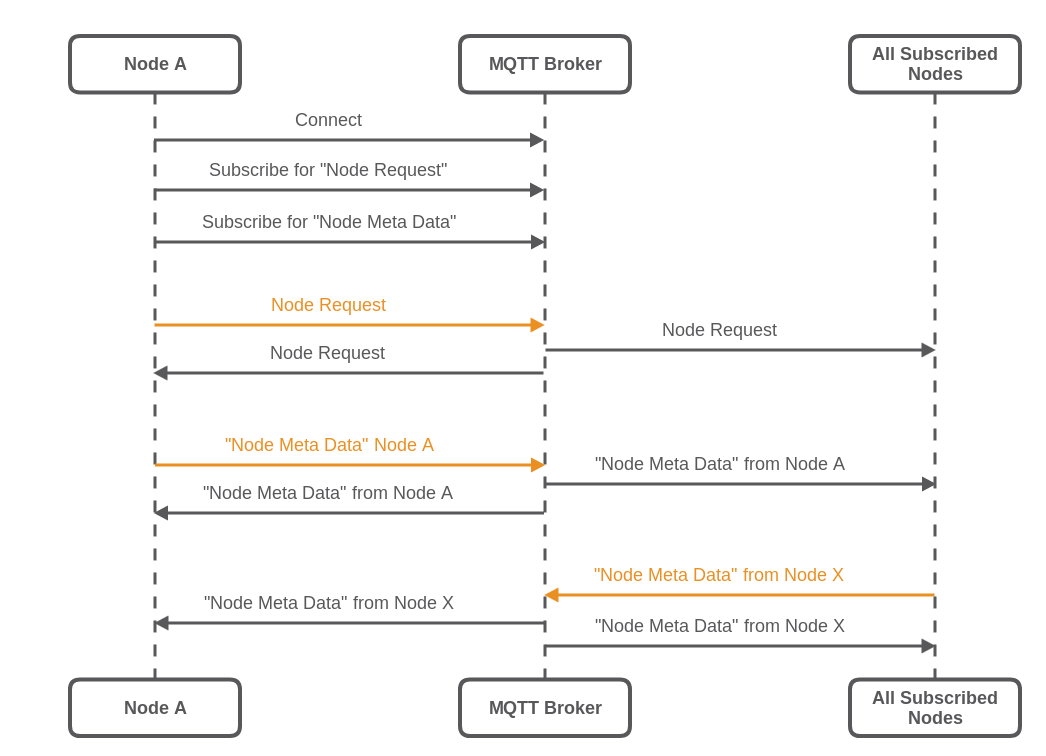
\includegraphics[width=\textwidth]{resources/images/node_discovery.png}
    \caption[Node discovery sequence diagram]{Node discovery sequence diagram}
    \label{fig:node_discovery_squ_dia}
\end{figure}

Figure \ref{fig:node_discovery_squ_dia} shows how the node discovery will be implemented.
Important aspect is that the sender node is also part of the subscribed nodes.
This means after the \textit{connection} to the broker is established and the client is subscribed to the topics, each \textit{Node Request} will also be received by the sender himself.
Benefit out of it, is that beside the fact that a new registered node gets all meta informations from all other nodes, also these nodes get the meta information of the new node.
In this way each node has knowledge of all the other nodes and can keep track of them.
That is also the reason why the \textit{"Node Meta Data" from Node A} and \textit{"Node Meta Data" from Node X} are duplicated in figure \ref{fig:node_discovery_squ_dia}.
Beside that the procedure is straight forward: At first one node send out a \textit{Node Request}.
Each subscribed node will get it and send out a response with the \textit{Node Meta Data} to all the other nodes via the broker.
The \textit{after\_connect} handler will be used to send out the \textit{Node Request} after a new nodes is sucessfully subscribed to the broker.
Before a node disconnects, a \textit{Remove Node} request will be send out, that will inform each node that a specific node will be disappear.
All the nodes react to this by removing the meta data about this node from the database.

\paragraph{ZeroMQServer}
Section \ref{section:ZeroMQ} and \ref{subsection:CommunicationLayer} gave a detailed overview about ZeroMQ and how does it work.
Now the concrete implementation will be discussed.
The wrapper class \textit{ZeroMQServer} binds multiple sockets to the related ports.
There are four sockets binded for the direct node-to-node communication via \ac{TCP} and one port to connect third party applications to the motey engine.
The latter is used to add or remove capabilies on a node.
ZeroMQ provides an \ac{IPC} protocol for such a use case.
The ZeroMQServer will bind a socket with the Publish-Subscribe pattern that allows multiple publisher to connect to the endpoint.
Two important aspects have to be considered by using the Publish-Subscribe pattern in ZeroMQ.
As in \ac{MQTT} each subscription has to be done to a topic.
Listing \ref{code:ZeroMQ-pub-sub} show the subscription for the \textit{capabilityevent} at line 3.
This also means that it is possible to send multiple different events to a single socket endpoint.
In motey this feature is not used yet, but nevertheless it is necessary to subscribe to a topic because of the implementation specification of ZeroMQ.
Without that, the subscriber will receive nothing.

\begin{listing}[H]
  \begin{minted}{python}
  def start(self):
    self.capabilities_subscriber.bind('ipc://*:%s' % config['ZEROMQ']['capability_engine'])
    self.capabilities_subscriber.setsockopt_string(zmq.SUBSCRIBE, 'capabilityevent')
    # [...]

  def __run_capabilities_subscriber_thread(self):
    while not self.stopped:
        result = self.capabilities_subscriber.recv_string()
        topic, output = result.split('#', 1)
        self.capability_event_stream.on_next(output)
  \end{minted}
  \caption{Example of the usage of the configreader}
  \label{code:ZeroMQ-pub-sub}
\end{listing}

The second important aspect is at line 9.
An incoming message has always been parsed for a delemiter.
The reason for that is, that the topic, in this case \textit{capabilityevent} have to be prepend to the message followed by the delimter.
Listing \ref{code:ZeroMQ-capability-event-msg} show such a message.
\begin{listing}[H]
  \begin{minted}{bash}
  capabilityevent#{'capability': 'zigbee', 'capability_type': 'hardware'}
  \end{minted}
  \caption{Example ZeroMQ capability event message}
  \label{code:ZeroMQ-capability-event-msg}
\end{listing}
Therefore the topics and the delimiter has to be removed before the message can be parsed.

The other four sockets are implemented with the Request-Reply pattern and are used to:
\begin{itemize}
  \item reply to a capability request.
  This is used by the \textit{inter\_node\_orchestrator} to get the capabilites of other nodes.
  The result is send as a \ac{JSON} string.
  If there are no capabilites an empty \ac{JSON} array will be send.
  \item deploy images is also used by the \textit{inter\_node\_orchestrator} to deploy a single image to another node.
  The image model will be transformed to a \ac{JSON} object and send over as a string and vice versa and passed over to the \textit{VALManager} if received.
  \item return the status of an image. \todo{write after implemented}
  \item termainate an existing image instance.
  Only the image id has to be send to perform that action.
  The \textit{VALManager} will handle the termination of the instance.
\end{itemize}
Important aspect while using the Request-Reply pattern, there can only be one connection established at the same time.
In addition a reply must send by the consumer after a request was receive.
As long as there was no message send back, the connection will be blocked and the consumer can not recevie any new messages.

As discussed by the other servers, also this one have to be executed in threads.
Difference here is that each socket has its own thread.
This is necessary because each connection waits for a request and has its own request loop.
Therefore each loop would block the main thread.

\paragraph{CommunicationManager}
Finally the \textit{CommunicationManager} is used to decorate the servers from the rest of the source code.
This is helpful for decoupeling the componants as well as replace or add a new communication component.
Beside that the manager simply forward the methods to the specific server.
It is also used as a central place to start and stop all servers.

\subsection{Capability management}
The main components of the capability management are the \textit{CapabilityEngine} and the \textit{ZeroMQServer}.
The latter was descibed in the previous section.


\subsection{User interface}
\doit

%\subsection{Deployment and Continous Integration}
% Travis.io
% Docker Container + Docker Hub
% setup.py
% Sphinx
%\doit

\section{Conclusion}
\doit
